\documentclass[11pt]{article}
\usepackage{graphicx} % graphic import stuff
\usepackage[parfill]{parskip} % to start each parapraph will an empty line before

%
% settings
%
\DeclareGraphicsExtensions{.pdf,.png,.jpg} % omits endings of graphics
\graphicspath{{./img/}} % the path to the graphics
%
% command for √ and x
%
\newcommand{\cmark}{\ding{51}}%
\newcommand{\xmark}{\ding{55}}%

%
% centers, scales and wraps a given graphic into a figure env
% % [1]: the scale factor 
% % [2]: the name of the image which will also be used with 'fig:' prefix as label
%% [3] the caption of the figure
%
\newcommand{\cgraphic}[4]
{
	\begin{figure}[htb]
		\begin{center}
		\includegraphics[scale=#1]{#2}
		\end{center}
		\caption{#3}
		\label{fig:#2}
	\end{figure}
}%

%opening
\title{Distributed Information Systems - Deliverable 1}
\author{Manuel Vogel, Felix Mohr,  Jinghua Lin}

\begin{document}
	\begin{titlepage}
		\centering
		
\includegraphics[width=0.5\textwidth]{hska-logo}\par\vspace{1cm}
		{\scshape\LARGE University of Applied Sciences - Karlsruhe \par}
		\vspace{1cm}
		{\scshape\Large Distributed Information Systems Lab\par}
		\vspace{1.5cm}
		{\huge\bfseries Deliverable 1 : Analysis of the legacy application\par}
		\vspace{2cm}
		{\Large\itshape Manuel Vogel, Felix Mohr,  Jinghua Lin\par}
		\vfill
		supervised by\par
		Prof~Dr.~Christian \textsc{Zirpins}
		\vfill
		{\large \today\par}
	\end{titlepage}
	
	\section{Start of the Webshop and functionality testing}
	Manu: Docker compose stuff
	
	\section{Analysis of the source code}
    Architecture and behavior: UML and class/sequence diagrams go here
    
    \subsection{Product management} % Felix
	The central module in product management are the classes \texttt{ProductManager} and \texttt{ProductManagerImpl}. Whenever a user action requires information concerning products, a method of this model will be invoked by the controller. The model does not directly use the database. It uses a Hibernate \textit{Data Access Object} for dealing with persistence tasks.

    When the user logs in, they have several options. One of them is listing all products using the \texttt{ListAll\-ProductsAction}.
    
    
		\begin{center}
		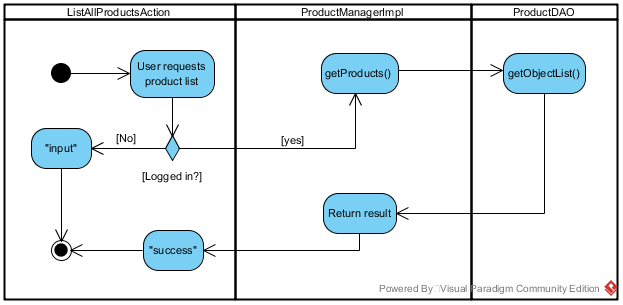
\includegraphics[width=\textwidth]{img/products/list}
		\end{center}
		
		
	For every product in the list, there is the possibility of showing its details. This action is being handled in the class \texttt{ProductDetailsAction}.
	\begin{center}
	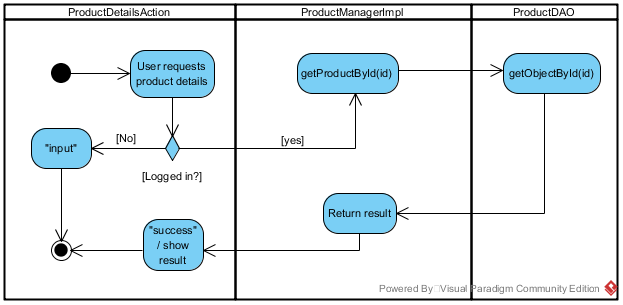
\includegraphics[width=\textwidth]{img/products/details}
	\end{center}
	
	Admins have additional possibilities. They are allowed to add/delete products and create/delete categories that products belong to.
	\begin{center}
	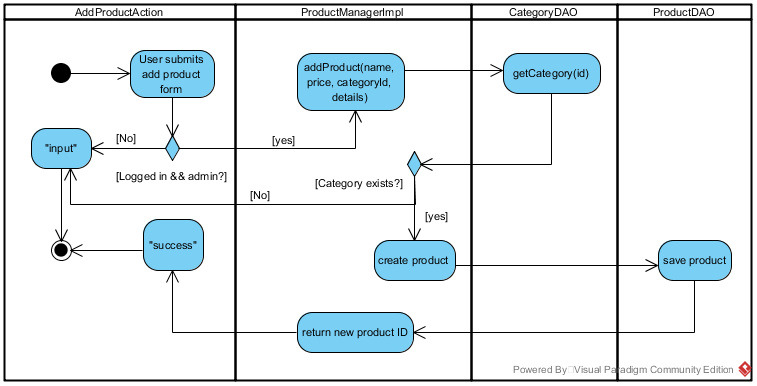
\includegraphics[width=\textwidth]{img/products/createproduct}
	\end{center}
	
	\begin{center}
	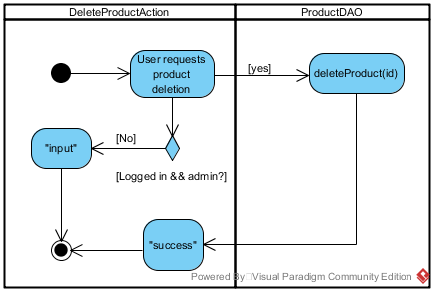
\includegraphics[width=0.7\textwidth]{img/products/deleteproduct}
	\end{center}
	
	\begin{center}
	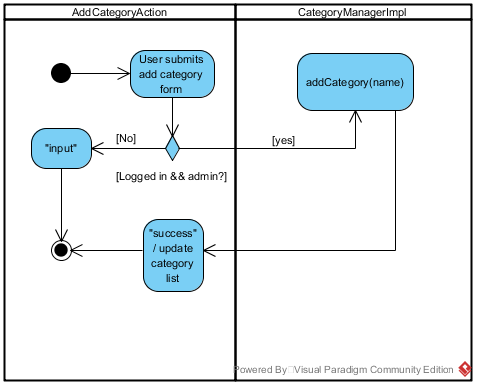
\includegraphics[width=0.7\textwidth]{img/products/addcategory}
	\end{center}
	
	The \texttt{DeleteCategoryAction} works just like the action used to delete a product, but it invokes the \texttt{CategoryDAO} instead of the product access object.
    
    \subsection{Search} % Manu
     
    \subsection{User management} %Lin
      
	
\end{document}
